%!TEX root =  ../main.tex
\renewcommand{\columnseprule}{1.5pt}
\begin{multicols*}{2}
\rule[0.5\baselineskip]{0.4\textwidth}{1pt}
\noindent
\LabSection{In the End}\label{sec:0601p}
\begin{exercises}{sec:0601p}
\lab{} Why are we able to predict the long-run behavior of any polynomial, simply by looking at the highest degree and leading coefficient?

\vspace{2cm}
\lab{} Complete the table below for any polynomial with the given quality of degree and given sign of leading coefficient.

%\vspace{1cm}
\noindent
\begin{tabular}{c | l | l}
	& \textbf{Positive} & \textbf{Negative} \\ \hline
	\textbf{Even} & $\displaystyle \lim_{x\rightarrow\infty}f(x)= \quad\quad\vspace{5mm} $ & $\displaystyle \lim_{x\rightarrow\infty}f(x)= \quad\quad\vspace{5mm} $\\
	& $\displaystyle \lim_{x\rightarrow-\infty}f(x)= \quad\quad\vspace{5mm} $& $\displaystyle \lim_{x\rightarrow-\infty}f(x)= \quad\quad\vspace{5mm} $\\ \hline
	\textbf{Odd} & $\displaystyle \lim_{x\rightarrow\infty}f(x)= \quad\quad\vspace{5mm} $ & $\displaystyle \lim_{x\rightarrow\infty}f(x)= \quad\quad\vspace{5mm} $ \\
	& $\displaystyle \lim_{x\rightarrow-\infty}f(x)= \quad\quad\vspace{5mm} $&$\displaystyle \lim_{x\rightarrow-\infty}f(x)= \quad\quad\vspace{5mm} $ \\
\end{tabular}  


\lab{} Recall that $y$-intercepts all have the form $(0,c)$, where $c$ is a Real number.  How can you easily look at any polynomial and tell what the $y$-intercept will be?

\vspace{2cm}
\lab{} Recall that $x$-intercepts all have the form $(c,0)$, where $c$ is a Real number.  If we have a polynomial in factored form, where are the $x$-intercepts?  For example, what are the intercepts of \\$f(x) = (x-3)(x+2)(2x-1)(x-5)$?

\vspace{3cm}
\lab{} What does it mean when a factor is repeated?  For example, what does $(x-1)^2$ look like?  What does $(x-1)^2(x+2)$ look like near $x=1$?

\vspace{2cm}
\noindent
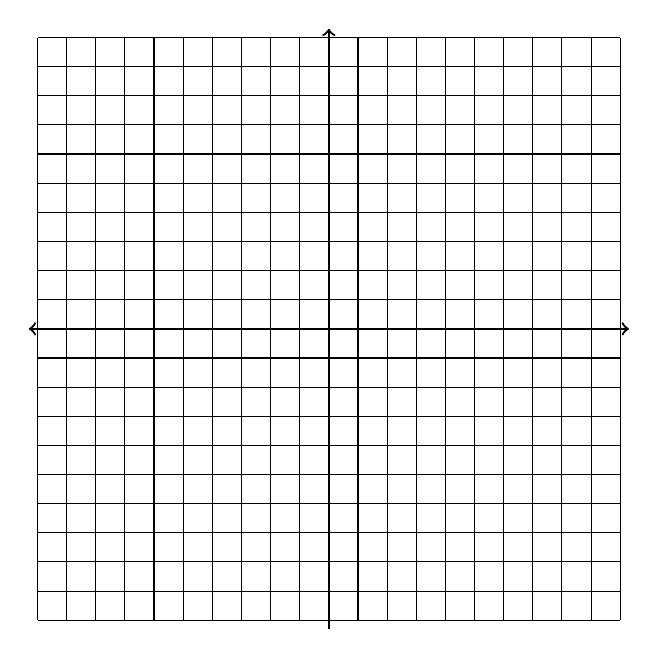
\begin{tikzpicture}[xscale=0.37,yscale=0.37]
	\draw [thick, <->] (-10.3,0) -- (10.3,0);
	\draw [thick, ->] (0,-10.3) -- (0,10.3);
	\draw [thin] (-10,-10) grid (10,10);
\end{tikzpicture}
\lab{} With all this information, we can sketch a graph of any polynomial.  Let us graph (without a grapher) the following function
$$
f(x) = -(x+1)^2(x-4)^2(3x+17)
$$
Begin by calculating what the leading term will be.  Do not multiply the entire equation out, only the $x$’s!

\vspace{1cm}
\lab{} This will allow you so determine the end-behavior.  Draw arrow beyond the left and right edges to indicate how the graph should ``end''.

\lab{} Calculate the constant-term.  Do not multiply the entire equation out, only the constants.  Mark the $y$-intercept, using a scale of 100:1.

\lab{} Mark the $x$-intercepts, noting whether they ``bounce'' or ``go through''.  Starting at the left edge of the graph and working write, sketch the entire function.

\lab{}  In technical language, describe what you think the point of this problem set it.
\end{exercises}
\end{multicols*}